\documentclass[a4paper,11pt]{article}
\usepackage{graphicx}
\usepackage{esvect}
\usepackage{subcaption}
\usepackage{listings}
\usepackage[top=0.75in, bottom=0.75in, left=0.6in, right=0.6in]{geometry}

\title{AE 625 - Particles Methods for Fluid Flow Simulation \\ SPH function and derivative approximation}
\author{Chillapalli Jyothi Durga Prasad - 140010042 }
\date{21 August 2017}

\usepackage{color}
 

\begin{document}
\maketitle


\tableofcontents
\listoffigures


\newpage
\section*{Consider the function −sin($\pi$x) in the region [-1, 1]. Sample this function at equal spaced intervals and perform an SPH approximation of the exact function.}
\indent The report is generated through the command \"\ sh a7-140010042.sh \"\\
\section{Plot the L2 error in the approximation with respect to the exact value as a function of the number of points used and the \'h\' value chosen. Use both a cubic spline kernel and the Gaussian Kernels. The L2 norm of a vector y is $|y|$=$(\sum{i}{} y_i)^{0.5}$. Perform the same for the derivative of the function and compare with the exact solution using the formula discussed..\\}


\textbf{Results:}\\

\indent \textbf{Cubic spline kernel}
\begin{figure}[ht]
    \centering
    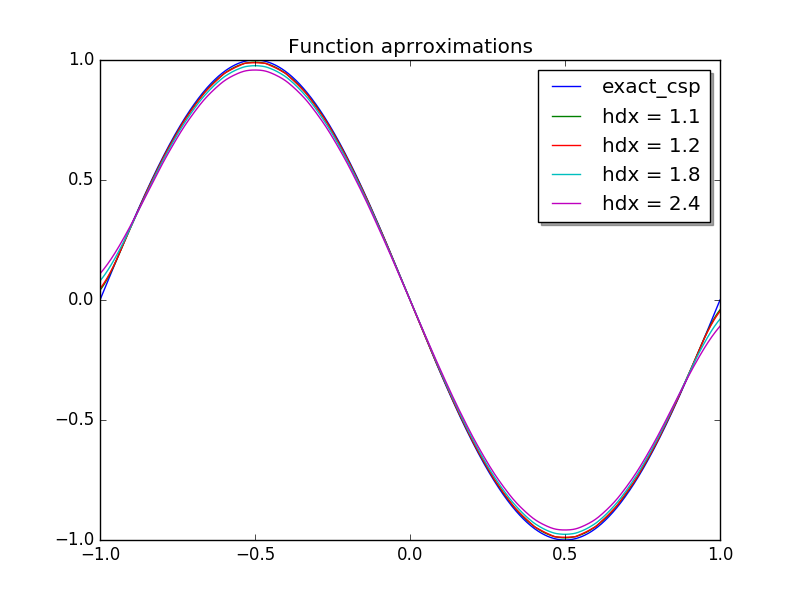
\includegraphics[width=.8\linewidth]{fun_csp.png}
    \caption{Cubic spline - function approx.}
    \label{fig:ex1}    
\end{figure}

\begin{figure}[ht]
    \centering
    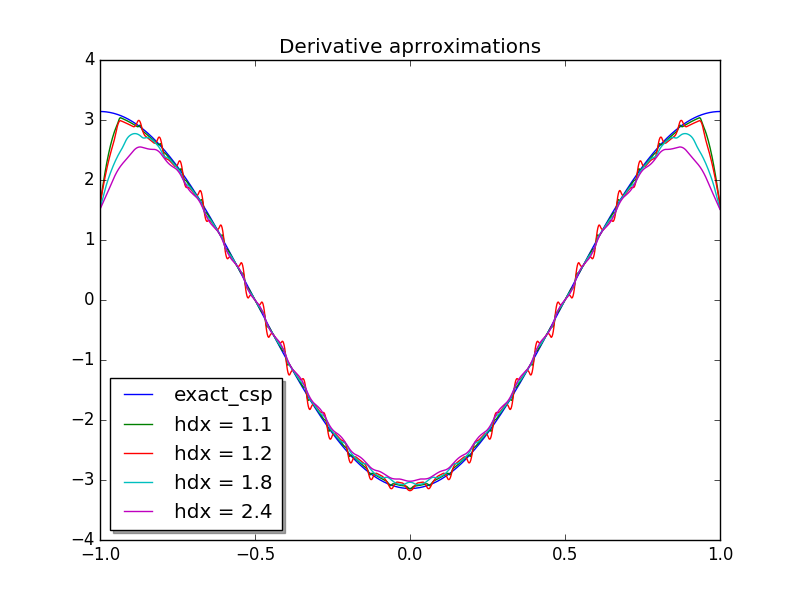
\includegraphics[width=.8\linewidth]{derv_csp.png}
    \caption{Cubic spline - derivative approx.}
    \label{fig:ex2}    
\end{figure}
\begin{figure}[ht]
    \centering
    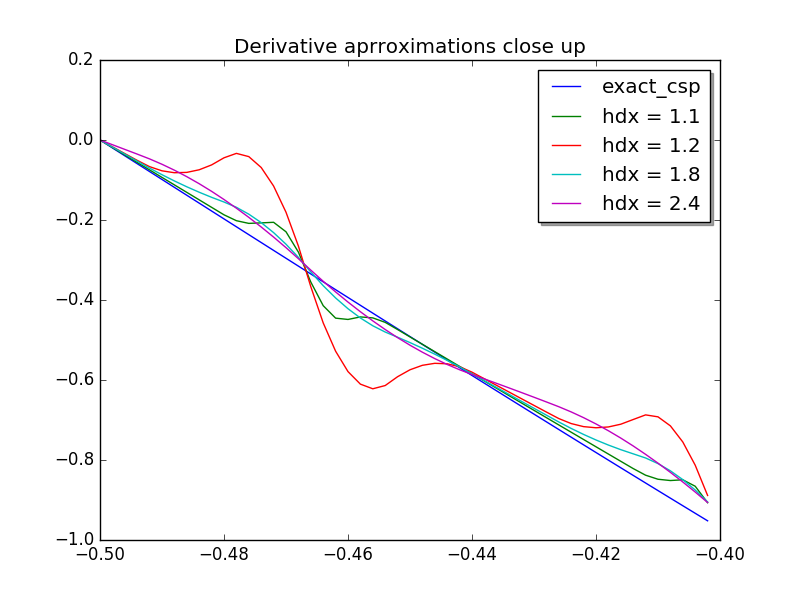
\includegraphics[width=.8\linewidth]{derv_csp_clup.png}
    \caption{Cubic spline - derivative approx close up.}
    \label{fig:ex3}    
\end{figure}

\begin{figure}[ht]
    \centering
    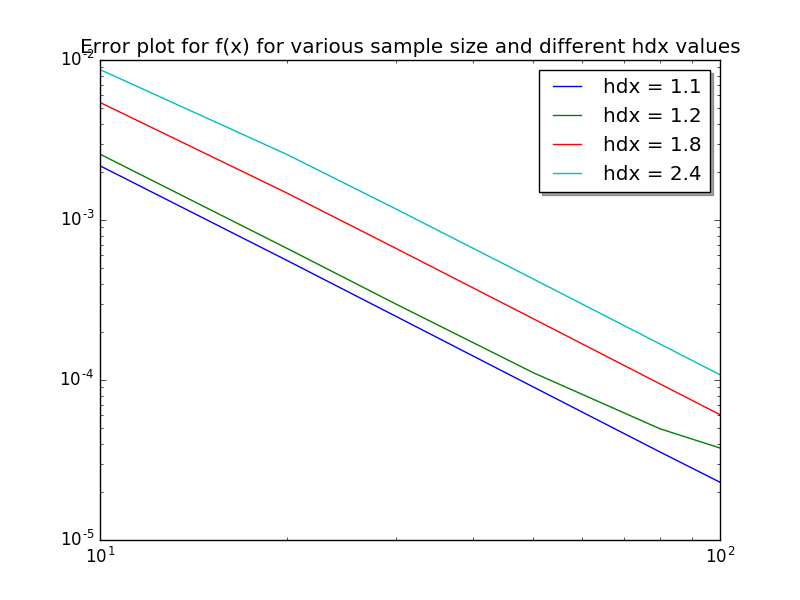
\includegraphics[width=.8\linewidth]{fun_err_csp.png}
    \caption{Cubic spline - function approx. error.}
    \label{fig:ex4}    
\end{figure}

\begin{figure}[ht]
    \centering
    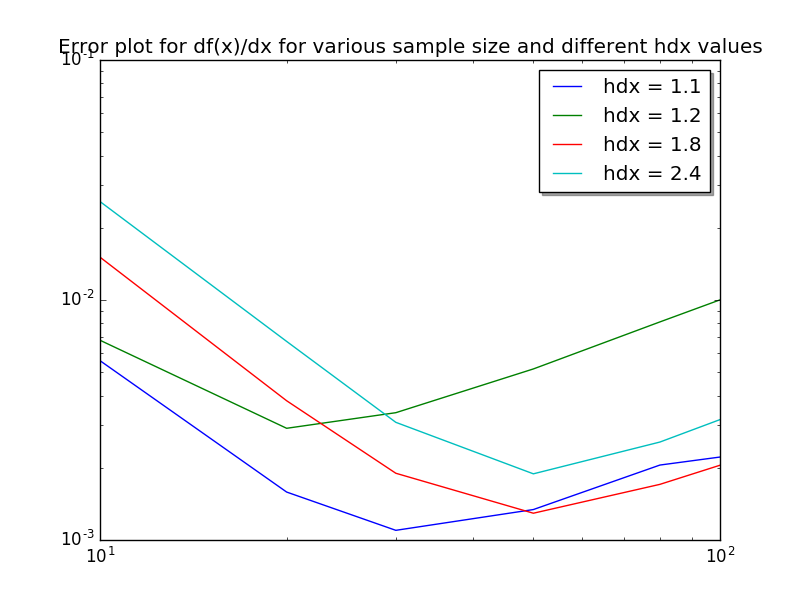
\includegraphics[width=.8\linewidth]{derv_err_csp.png}
    \caption{Cubic spline - derivative approx. error.}
    \label{fig:ex5}    
\end{figure}


\newpage
\indent\\
\newpage
\indent\\
\newpage
\indent\\
\newpage
\indent\\
\newpage
\indent\\


\indent \textbf{Gaussian kernel}
\begin{figure}[ht]
    \centering
    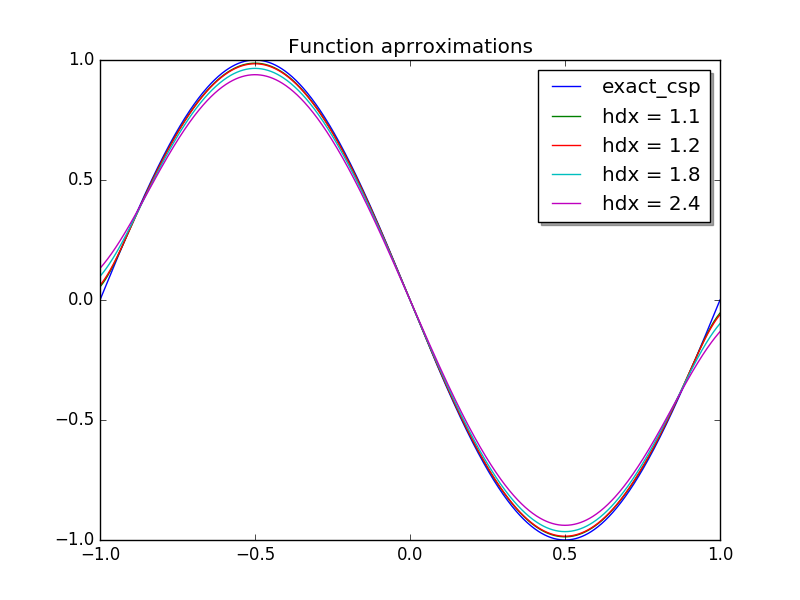
\includegraphics[width=.8\linewidth]{fun_gau.png}
    \caption{Gaussian - function approx.}
    \label{fig:ex6}    
\end{figure}

\begin{figure}[ht]
    \centering
    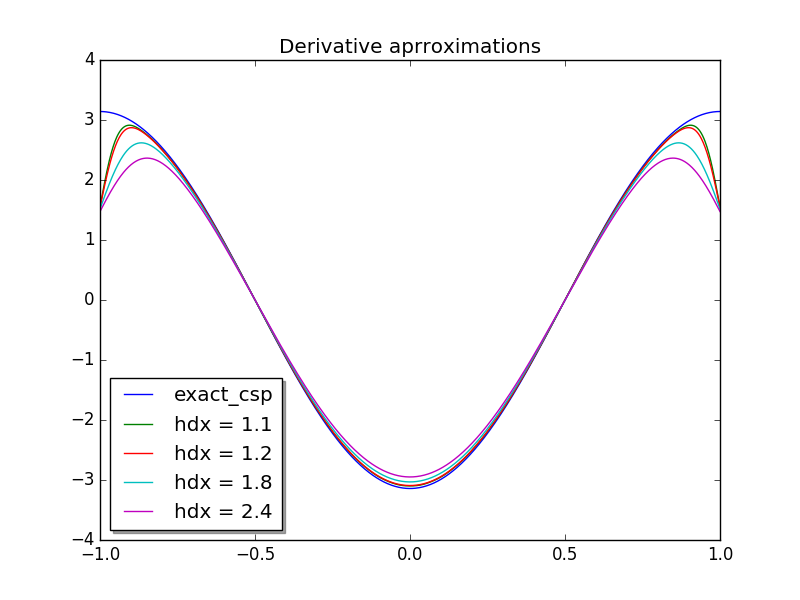
\includegraphics[width=.8\linewidth]{derv_gau.png}
    \caption{Gaussian - derivative approx.}
    \label{fig:ex7}    
\end{figure}
\begin{figure}[ht]
    \centering
    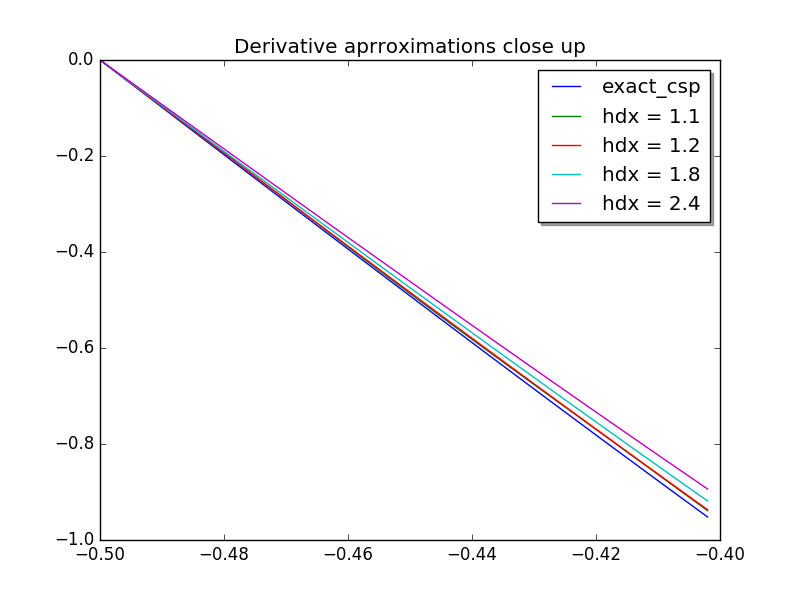
\includegraphics[width=.8\linewidth]{derv_gau_clup.png}
    \caption{Gaussian - derivative approx closeup.}
    \label{fig:ex8}    
\end{figure}

\begin{figure}[ht]
    \centering
    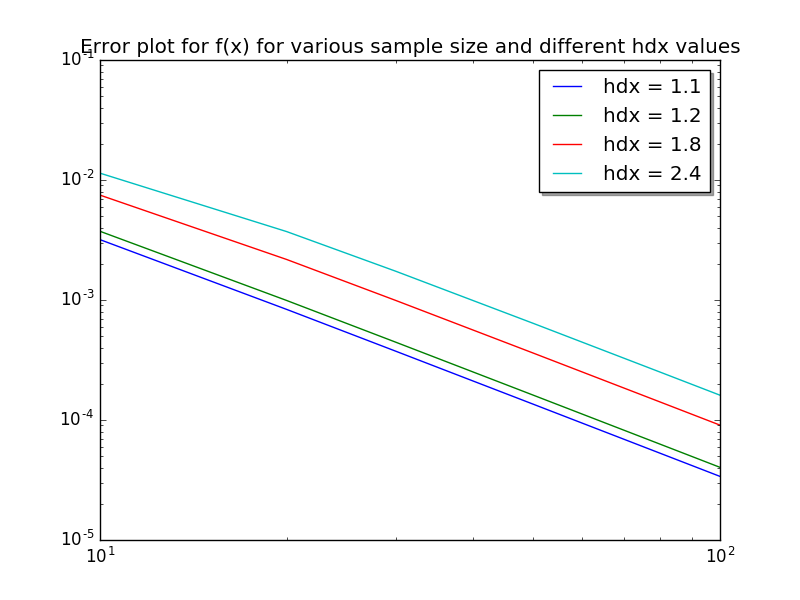
\includegraphics[width=.8\linewidth]{fun_err_gau.png}
    \caption{Gaussian - function approx. error.}
    \label{fig:ex9}    
\end{figure}

\begin{figure}[ht]
    \centering
    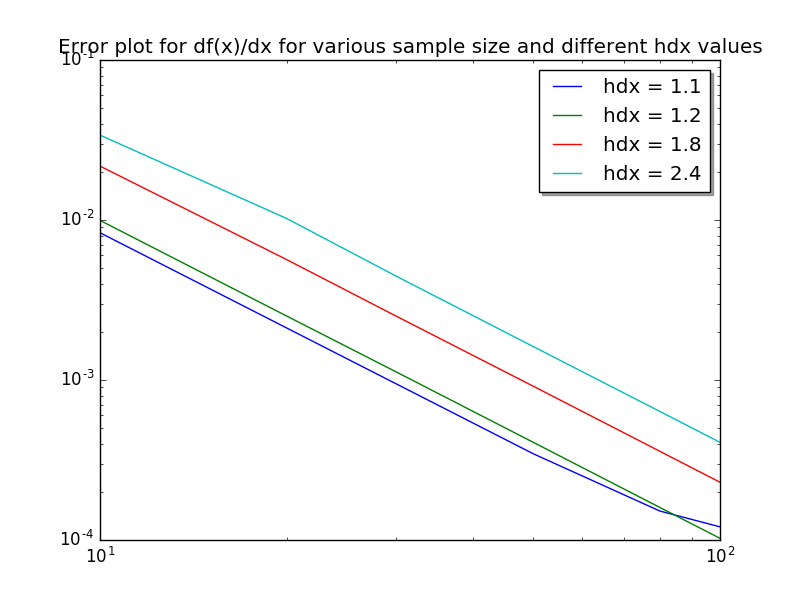
\includegraphics[width=.8\linewidth]{derv_err_gau.png}
    \caption{Gaussian - derivative approx. error.}
    \label{fig:ex10}    
\end{figure}

\begin{figure}[ht]
    \centering
    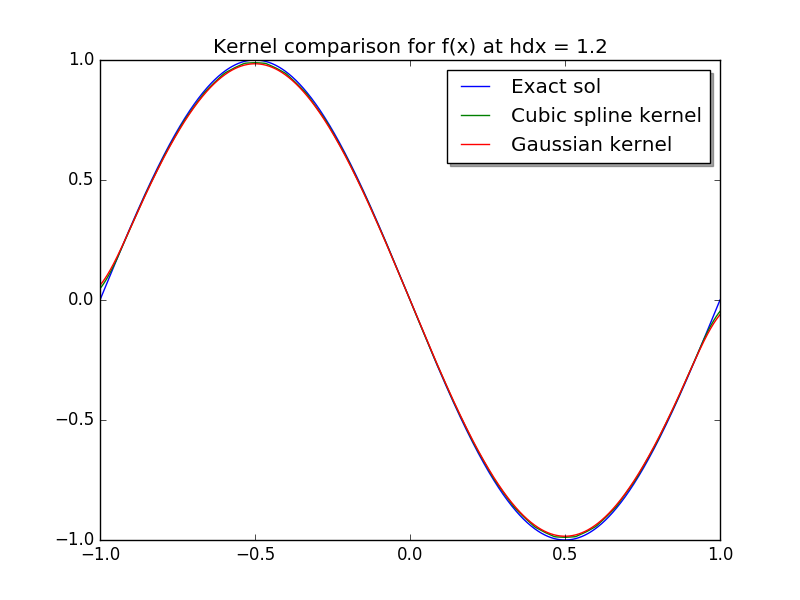
\includegraphics[width=.8\linewidth]{comp_fn.png}
    \caption{Kernel comparison - function approx. }
    \label{fig:ex9}    
\end{figure}

\begin{figure}[ht]
    \centering
    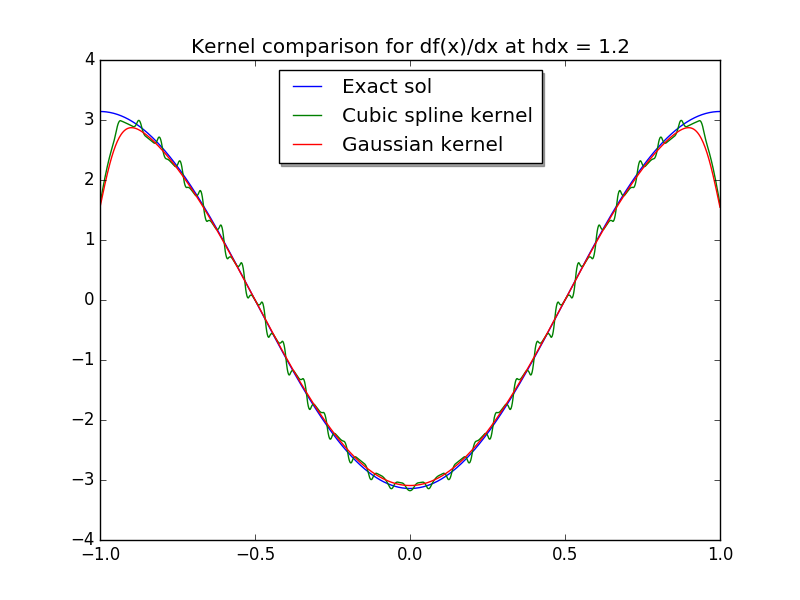
\includegraphics[width=.8\linewidth]{comp_dfn.png}
    \caption{Kernel comparison - derivative approx.}
    \label{fig:ex10}    
\end{figure}

\newpage
\indent\\
\newpage
\indent\\
\newpage
\indent\\
\newpage
\indent\\
\newpage
\indent\\
\newpage
\indent\\

\section{Finally, pick one of the kernels and add a small amount of noise to the positions of the particles (by adding a small random displacement, uniformly distributed), and see how this affects the accuracy.}

\textbf{Results:}

\indent Approximation without noise for hdx = 1.1 .
\begin{figure}[ht]
    \centering
    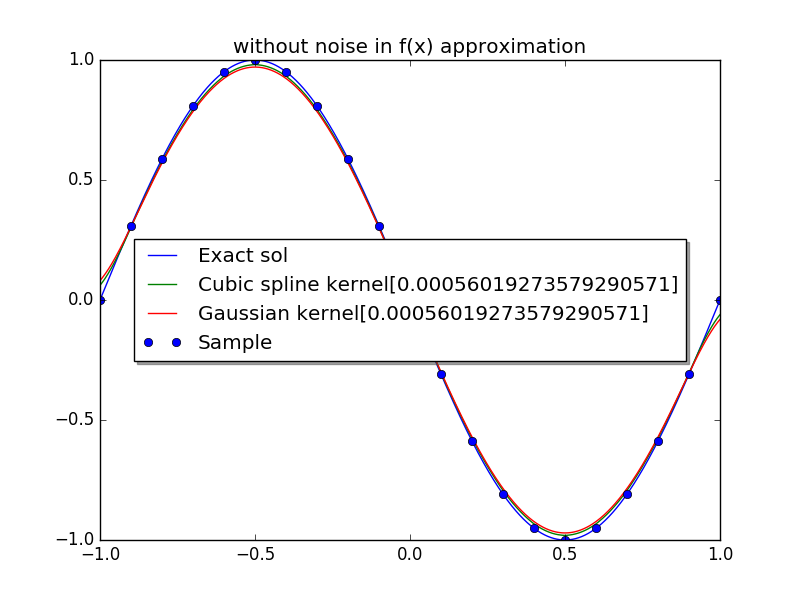
\includegraphics[width=.8\linewidth]{nnoise.png}
    \caption{function approx without noise}
    \label{fig:ex11}    
\end{figure}

\begin{figure}[ht]
    \centering
    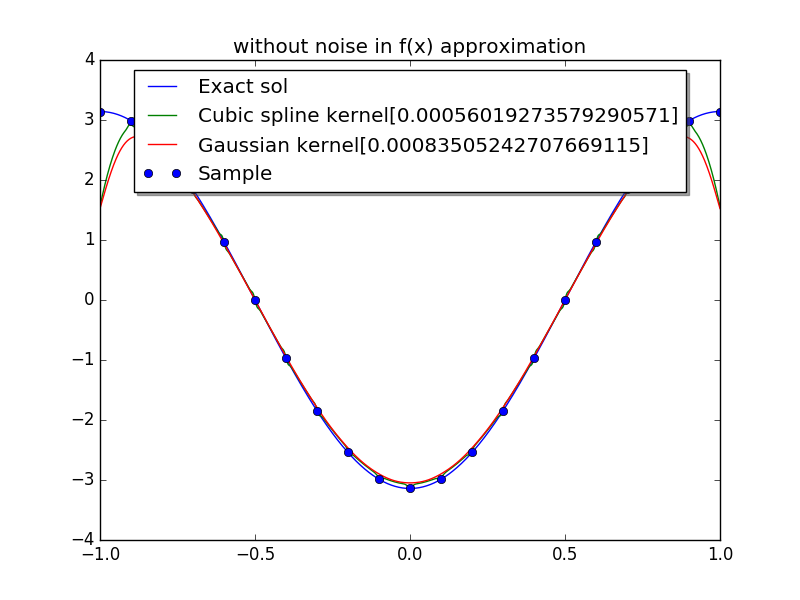
\includegraphics[width=.8\linewidth]{ndnoise.png}
    \caption{derivative approx without noise}
    \label{fig:ex12}    
\end{figure}
\newpage
\indent\\
\newpage
\indent\\
\newpage
\indent\\
\indent Approximation with noise for hdx = 1.1 .
\begin{figure}[ht]
    \centering
    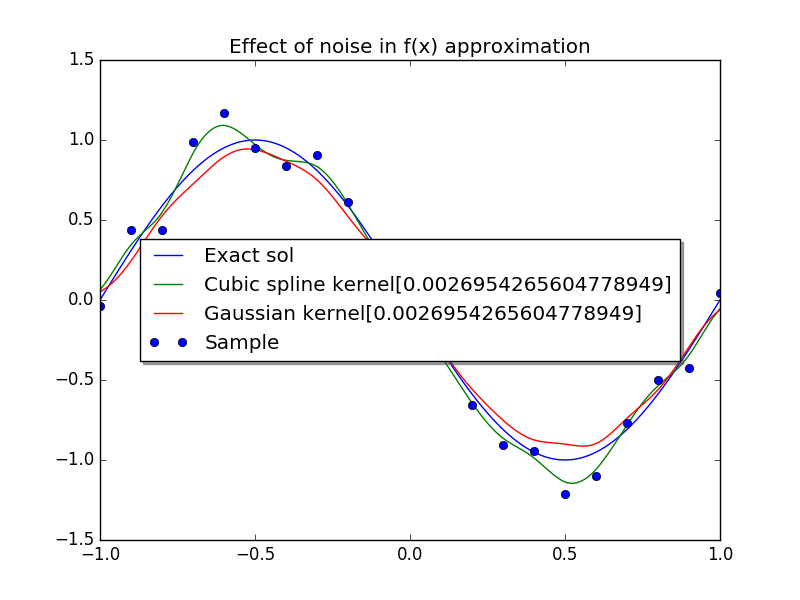
\includegraphics[width=.8\linewidth]{noise.png}
    \caption{function approx with noise}
    \label{fig:ex13}    
\end{figure}

\begin{figure}[ht]
    \centering
    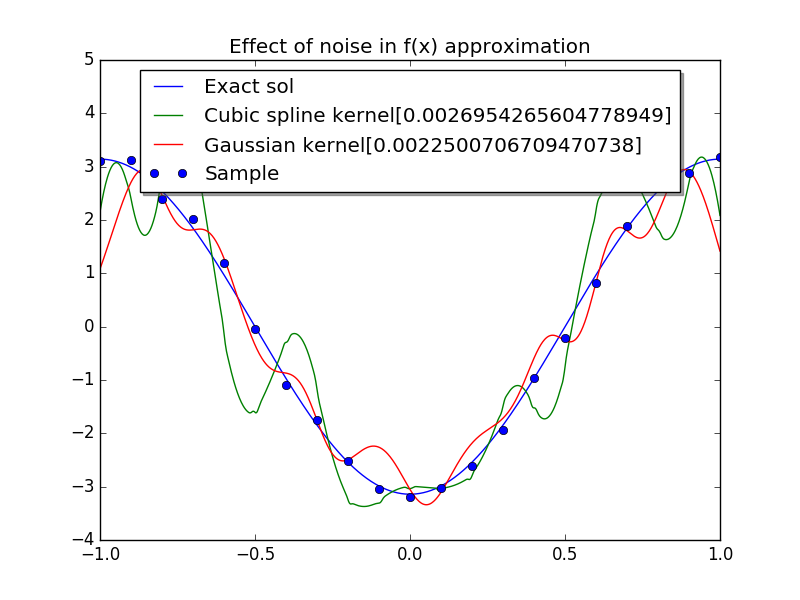
\includegraphics[width=.8\linewidth]{dnoise.png}
    \caption{derivative approx with noise}
    \label{fig:ex14}    
\end{figure}
\end{document}
